%%%%%%%%%%%%%%%%%%%%%%%%%%%%%%%%%%%%%%%%%%%%%%%%%%%%%%%%%%%%%%%%%%%%%%%%%%%%%%%%
%2345678901234567890123456789012345678901234567890123456789012345678901234567890
%        1         2         3         4         5         6         7         8

\documentclass[letterpaper, 10 pt, conference]{ieeeconf}  % Comment this line out
                                                          % if you need a4paper
%\documentclass[a4paper, 10pt, conference]{ieeeconf}      % Use this line for a4
                                                          % paper

\IEEEoverridecommandlockouts                              % This command is only
                                                          % needed if you want to
                                                          % use the \thanks command
\overrideIEEEmargins
% See the \addtolength command later in the file to balance the column lengths
% on the last page of the document



% The following packages can be found on http:\\www.ctan.org
\usepackage{graphics} % for pdf, bitmapped graphics files
\usepackage{graphicx}
%\usepackage{epsfig} % for postscript graphics files
%\usepackage{mathptmx} % assumes new font selection scheme installed
%\usepackage{times} % assumes new font selection scheme installed
% \usepackage{amsmath} % assumes amsmath package installed
% \usepackage{amssymb}  % assumes amsmath package installed

\title{\LARGE \bf
Effects of Corpus Variation on LDA
}

\author{ \parbox{3 in}{\centering \textbf{Cassian J. Corey} \\
        University of Massachusetts Amherst\\
        {\tt\small cjcorey@umass.edu}}
        \hspace*{ 0.5 in}
}

% \author{Huibert Kwakernaak$^{1}$ and Pradeep Misra$^{2}$% <-this % stops a space
% \thanks{*This work was not supported by any organization}% <-this % stops a space
% \thanks{$^{1}$H. Kwakernaak is with Faculty of Electrical Engineering, Mathematics and Computer Science,
%         University of Twente, 7500 AE Enschede, The Netherlands
%         {\tt\small h.kwakernaak at papercept.net}}%
% \thanks{$^{2}$P. Misra is with the Department of Electrical Engineering, Wright State University,
%         Dayton, OH 45435, USA
%         {\tt\small p.misra at ieee.org}}%
% }


\begin{document}

\maketitle
\thispagestyle{empty}
\pagestyle{empty}


%%%%%%%%%%%%%%%%%%%%%%%%%%%%%%%%%%%%%%%%%%%%%%%%%%%%%%%%%%%%%%%%%%%%%%%%%%%%%%%%
\begin{abstract}

This project explores the effects of corpus modification on the performance of topic modeling techniques. Corpora gathered from NLTK are modified and topics are extracted using Latent Dirichlet Allocation. We find that the quality of topics extracted from a corpus rely on more than just a few basic corpus properties. In addition to confirming the existing results on topic model evaluation, we make several substantial contributions to the work of evaluating topic modeling and showing the effects of corpus properties on the metrics used to evaluate models.

\end{abstract}


%%%%%%%%%%%%%%%%%%%%%%%%%%%%%%%%%%%%%%%%%%%%%%%%%%%%%%%%%%%%%%%%%%%%%%%%%%%%%%%%
\section{INTRODUCTION}

Publishing and sharing digitized text on the Internet is becoming increasingly popular. Online books, news articles, social media outlets, question-answer forums, and many other sources are generating a wide variety of new corpora for researchers to study. Often, the trouble with such large amounts of documents is that no one knows where to begin.

Topic modeling addresses this issue by identifying themes among large sets of documents. Most approaches to topic modeling rely on the underlying phenomena of word co-occurrences to generate topics. In this work, we aim to explore the relationship between this phenomena and the topics produced by topic modeling. In particular, we address two research questions:
\begin{itemize}
\item What observable properties exist in real-world corpora and what is their relationship to the topics in these corpora?
\item What effect does modification of these properties have on the quality of topics being produced?
\end{itemize}

In addition to re-iterating some of the findings of \cite{tang2014understanding}, we make the following observations:
\begin{itemize}
\item Some real-world corpus properties (such as number of documents and vocabulary size) vary drastically while others (such as stopword presence) do not.
\item This natural bound of stopword presence creates a threshold for the effect of stopword injection and removal on cosine distance between topics.
\item Easier-to-compute topic metrics (as opposed to coherence and perplexity on held-out data) exist that can still confidently distinguish between strong and weak topics.
\end{itemize}

\section{RELATED WORK}

\subsection{Topic Modeling}
There has been extensive work to develop and revise various approaches to topic modeling. The literature has mostly agreed that Latent Dirichlet Allocation (LDA) \cite{blei2003latent} is one of the best approaches. In its most baseline form, LDA still requires several input variables before it can be fit to a corpus. To fix the model, it is necessary to fix the number of topics (K), the prior distribution of topics within documents ($\alpha$), and the prior distribution of words within topics ($\beta$). Previous work has shown that the model performs best with asymmetric $\alpha$ and symmetric $\beta$ \cite{wallach2009rethinking}. In \cite{tang2014understanding}, it was shown that the posterior contraction rate of topic distributions is independent of the number of topics. Therefore, it is only necessary to choose K to be sufficiently high enough for the model to separate any topics present in the corpus.

Topic modeling addresses the desire to improve user experience when encountering large availability of text documents. The generative model Latent Dirichlet Allocation (LDA) is currently the most widely used topic modeling algorithm. First introduced by \cite{blei2003latent}, LDA identifies latent topics within discrete datasets by considering each topic to be a multinomial distribution over the words in the vocabulary. In turn, each document is composed of topics sampled from a Dirichlet distribution over the topic-space. LDA was successful at addressing issues that previous models had with over-fitting, unrealistic increases in parameter counts, and infeasible run-times \cite{blei2003latent}.

Following its arrival, LDA was applied to many situations both with and without success. For more than a decade, there was only a casual understanding of which situations were well-suited to LDA and which were not. Researchers made ad-hoc changes to the model to suit the properties of their corpus. They gave minimal consideration to how these changes would generalize to other types of data. For example, researchers soon discovered that LDA was ill- suited to documents that were too short (such as tweets) and documents that were too long, with too many topics (such as books). \cite{mimno2007organizing} addresses the issue of documents being too long and containing too many topics with DCM-LDA, a model which they tested on 1.4 billion words and more than 12,000 topics. However, their claims for generalization apply only to increases in the size of the corpus, the length of documents, and the number of topics. They do not address changes in the other direction. This is left to others such as the modified LDA models seen in \cite{zuo2016topic,zhao2011comparing}. They only test and evaluate their new method on the specific type of document it was designed to address.

Tang et al. \cite{tang2014understanding} provided the first deliberate study of LDA parameters and their limitations as well as the specific properties that make a dataset well-suited for LDA. Their experiments specifically focused on measuring the contraction rate of topics around the true topic-space center as the number of documents and size of each document increases to infinity. Results showed the importance of choosing the correct number of topics and setting the Dirichlet priors to large or small values depending on the number of topics associated with each document.

Despite a near-complete understanding of LDA’s limiting factors after \cite{tang2014understanding}, research is still missing the mark as publications continue to show modifications being fine-tuned to specific datasets \cite{zuo2016topic}. Consistent, generalized methods for how to construct better documents and evaluate resulting models are lacking.

\subsection{Word Co-Occurrence}

It is well-understood that co-occurrence of words is the underlying phenomenon that defines a topic \cite{tang2014understanding,zuo2016topic,zhao2011comparing,mimno2007organizing}. Future work should utilize this knowledge when deciding how to generate appropriately sized documents during preprocessing. In addition, if modifications to LDA are going to continue, we need a consistent method for evaluating model performance. Currently, classification tasks and comparison against ground-truth topic labels are the only two methods used. These are risky methods because ground-truth is not always available and generating labels for datasets is not always feasible.

\subsection{Measuring Topic Quality}

There is an often overlooked but rather obvious end-goal of topic modeling: distinguishing ``good'' from ``bad'' topics. Whether they know where to start or not, a user faced with large amounts of data and presented with several potential starting points will always be able to distinguish the ``strong'' starting points from the ``weak.'' Understanding what makes some topics strong (or interesting) and other topics weak (or uninteresting) is key to evaluating the different extensions of generic LDA.

Most publications already include some sort of quality measure for individual topics and distance measures for comparing topics or topic-spaces. All use topic coherence to establish a quality for topics. Zhao uses human subjects to score topic quality (an insightful method although it does not scale well). Jensen-Shannon Distance is used by \cite{mimno2007organizing,zhao2011comparing,zuo2016topic} to compare topics within the same topic-space and by \cite{tang2014understanding} to compare topics from different topic-spaces. The only missing step is to take these similar approaches and conduct one formal method for evaluating derived topic qualities.

\section{EXPERIMENTAL DESIGN}

\subsection{Choosing Corpora}

Corpora were chosen based on their availability with slight attention to ensuring a wide variety of corpus properties. Five real-world corpora were chosen: Wine, ABC Science, ABC Rural, and Brown. Brown is perhaps one of the most famous and widely used corpora. It was the first digital corpora and is regarded as a good sample of the American English language. ABC Science is a collection of scientific articles from ABC News. ABC Rural is its non-scientific counterpart. Wine is a collection of wine reviews.

\begin{table}[ht]
\renewcommand{\arraystretch}{1.3}
\caption{Directly Varied Corpus Properties}
\label{corpus_properties}
\centering
\begin{tabular}{c||l|l|l|l}
\hline
\bfseries Corpus & \bfseries \# Docs & \bfseries Doc. Len. & \bfseries S.W. \% & \bfseries Vocab. Size \\
\hline\hline
ABC Science & 764 & 551 & 0.35 & 24306\\
ABC Rural & 2424 & 143 & 0.35 & 17222\\
Brown & 500 & 2418 & 0.37 & 48675\\
Wine & 1230 & 25 & 0.26 & 3414\\
\hline
\end{tabular}
\end{table}

Table \ref{corpus_properties} shows the corpora and their properties. We chose to measure and modify the number of documents, the average document length (in words), and the presence of stopwords.

The number of documents and average document length were chosen due to their frequency of being mentioned and tampered with in related work on topic modeling. Calculating these properties is straightforward.

Stopword presence represents the percentage of the corpus that is made up of stopwords found in the NLTK list of English stopwords \cite{NLTK}.

In preliminary experiments we also tested lexical diversity, readability, vocabulary size, and distance of the bag-of-words representation of documents from a uniform distribution over the corpus vocabulary. Although interesting, lexical diversity and readability rely on punctuation to score text. Since our chosen topic modeling algorithm views documents as bags-of-words, these two were not feasible options for modification. We reason that vocabulary size and the distance of documents from a uniform distribution over the vocabulary size are both affected by the presence of stopwords. Furthermore, presence of stopwords is easy to manipulate. For these reasons, we chose to expand on existing work by modifying the presence of stopwords in our chosen corpora.

\subsection{Varying Corpus Properties}

\subsubsection{Number of documents and document length}
To vary the number of documents, a uniform random selection of documents was made ranging from 10-100\% of the original corpus. The number of words in each document was similarly varied by making a uniform random selection of 10-100\% of the words from each document.

\subsubsection{Presence of stopwords}
To alter the presence of stopwords in each document, we begin by finding the intersection between NLTK's list of English stopwords and the words present in the document. Then, we randomly remove or inject stopwords from that list until anywhere from 0\% to 90\% of the document is composed of stopwords. Since the topic model uses a bag-of-words approach, we do not need to worry about where stopwords are being removed from or injected into the document.

\subsection{A Fixed Approach to Topic Modeling}

After manipulating corpus properties, we extract topics using a fixed model. Our model is uses Latent Dirichlet Allocation to extract topics. It extracts K=15 topics with symmetric document-topic ($\alpha$) and topic-word ($\beta$) priors both set to 1/K. Determining the true number of topics in a corpus is an inherently difficult task, and increasing the number of topics also increases runtime of the algorithm. Therefore, we believe K=15 is a reasonable number of topics to observe the behaviour we are looking for.

\subsection{Measuring Topic Quality}

Extracted topics need to be measured for quality. The most popular forms of topic evaluation today rely on UCI coherence and the model’s perplexity on held-out documents. UCI coherence requires collecting external word co-occurrence data from Wikipedia (or other wiki-type sources) and perplexity requires having or obtaining labels for the true underlying topics. Unfortunately, these tasks are both out of the scope of this project as they require significant extra work.

We propose several new topic metrics that do not rely on external information or ground-truth labeling. Each metric is designed to satisfy the following three axioms:
\begin{enumerate}
\item Similar topics should have similar scores
\item Different topics should have different scores
\item Changing the underlying topic word-likelihoods should also change the score
\end{enumerate}

The metrics are: distance from uniform distribution, effective size, exclusivity, and rank1. The equations for these metrics are mainly obtained from \cite{mallet2002} which provides detailed instructions for calculating each metric as well as how to interpret the value.

\subsubsection{Distance from uniform} A topic's distance from the uniform distribution over the corpus vocabulary space is calculated using Kullback-Leibler divergence. Also known as the relative entropy, Kullback-Leibler divergence measures the information gain of using the topic to construct a document versus using the uniform distribution over the vocabulary space or the observed distribution of vocabulary words in the corpus. We want topics that diverge from the corpus and uniform distributions because that means they stand out and are more descriptive than those that converge.

\subsubsection{Effective size} Effective size is equivalent to the effective number of parties measure used in politics. It weighs each word in a topic by the words relative likelihood of being found in that topic. The result is that topics comprised of a few extremely likely words are effectively smaller than topics comprised of many equally likely words. Topics that are more broad will have a larger effective size. Therefore, we say a topic is good if it has a relatively small effective size (when compared to the other topics).

\subsubsection{Exclusivity} Exclusivity measures the degree to which top words in one topic also appear as top words in another topic. First, we take the likelihood of each top word in a topic and divide it by the sum of the likelihoods of that word in all other topics. The average of this fraction over all top words in a topic is that topic’s exclusivity.

\subsubsection{Rank1} In LDA, documents can contain several topics. Rank1 counts the number of documents that rank a given topic as their most common topic. The higher this metric is, the worse a topic is. Topics that are very popular in a lot of documents are probably meaningless because they are so popular. They will not stand out as much as a topic that is only spoken about frequently in a small subset of documents.

\subsubsection{Cosine Distance} Unlike the previous metric, this one deals with topics in pairs. LDA represents topics as vectors of word-likelihoods and topic-word prior guarantees that these vectors are non-zero for every topic. This makes it possible to calculate topic similarity using cosine distance for every pair of topics produced by the model.

\subsubsection{Jensen-Shannon and Kullback-Leibler Divergence} These two metrics are both measures of topic similarity, like cosine distance. Both measure the similarity between topics represented as probability distributions. Jensen-Shannon divergence is the symmetric version of Kullback-Leibler divergence.

\subsection{Challenges}

One of the challenges of performing multiple iterations of Latent Dirichlet Allocation is that it does not maintain consistent topic ordering. Asking which topic is which across multiple iterations on the same corpus is in some ways the wrong question to ask. A better question would be to ask which topics most closely resemble other topics and at what point do they become impossible to distinguish. A metric such as cosine distance could be used to pair topics across iterations. However, we are explicitly seeking to test the degradation or topics. It is destined to become an impossible task.

Instead of attempting to ``match'' topics, we decided that the best method would be to plot the results in a way that made pairs obvious to the human observer. For this reason, all of our plots are scatter plots. Although we cannot say with complete confidence that the data points you see following a specific trend represent the same topic over the iterations, it is very likely that from a human interpretation, they are the ``same'' topic. In fact, we intentionally designed our topic metrics with this difficulty in mind (see previous section on ``Measuring Topic Quality'').

\section{RESULTS}

In all plots, topic metrics have been scaled to fit all four corpora on the same plot. We ensured beforehand that scaling does not affect the outcomes.

\subsection{Number of Documents}

\subsubsection{Distance from Uniform} As the number of documents increases, we observe an increase in topic distance from the uniform distribution. This increase is minor for the majority of topics but quite severe for those weaker topics that contain mostly corpus stopwords. Increasing the document length only adds to the effect, pushing topics farther from the uniform distribution. Increasing the stopword presence slightly increases variance of the scores for most topics but most severely impacts the weaker topics. At 90\% stopword presence, the weakest topic is clearly distinguishable from the remainder of topics regardless of the number of documents in the corpus or their length. 

\subsubsection{Effective Size} The effect of increasing the number of documents in the corpus on effective size of topics is shown in Figure \ref{fig:nd_eff_size}. There is a logarithmic relationship of the form $y=a*\log(x)+b$ between the number of documents and the effective size of topics where $\log(x)$ is the natural $\log$ (base $e$) of $x$.
\begin{figure}[thpb]
      \centering
      \framebox{
      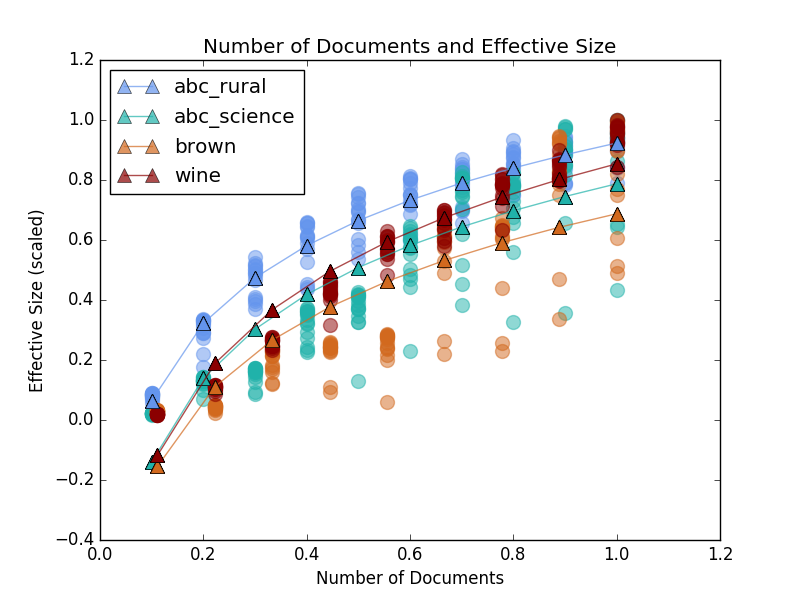
\includegraphics[width=3.0in]{num_docs_eff_size_fitted.png}
	  }
      \caption{Effect of manipulating number of documents in corpus on effective size of topics}
      \label{fig:nd_eff_size}
\end{figure}

\subsubsection{Exclusivity} As the number of documents increases, exclusivity of topics increases exponentially. This can be seen in Figure \ref{fig:nd_exclusivity}. 
\begin{figure}[thpb]
      \centering
      \framebox{
      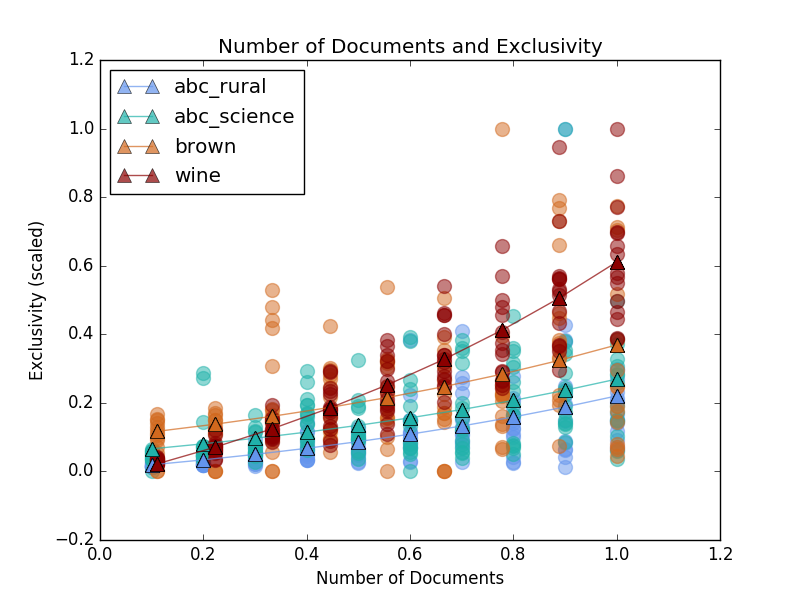
\includegraphics[width=3.0in]{num_docs_exclusivity_fitted.png}
	  }
      \caption{Effect of manipulating number of documents in corpus on topic exclusivity}
      \label{fig:nd_exclusivity}
\end{figure}

\subsubsection{Rank1} Rank1 shows a slight exponential increase with the increase in number of documents for all four corpora. Figure \ref{fig:nd_rank1} shows these results. On top of increasing corpus size through number of documents, increasing the presence of stopwords in these documents decreases the strength of the relationship between Rank1 and number of documents. Increasing the length of these documents does not affect the parameters of the relationship.
\begin{figure}[thpb]
      \centering
      \framebox{
      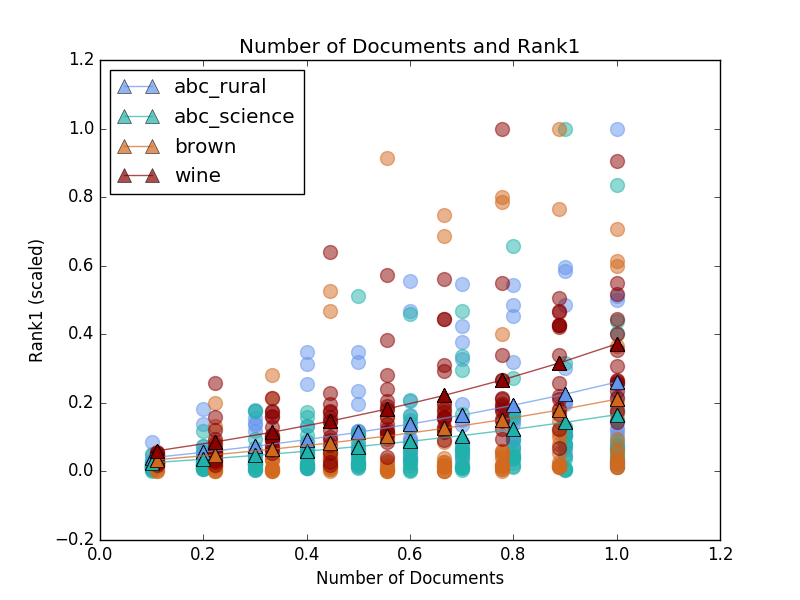
\includegraphics[width=3.0in]{num_docs_rank1_fitted.png}
	  }
      \caption{Effect of manipulating number of documents in corpus on topic rankings within documents}
      \label{fig:nd_rank1}
\end{figure}

\subsubsection{Cosine Distance} The results of modifying the number of documents on cosine distance are shown in Figure \ref{fig:nd_cos}. There is a subtle positive logarithmic correlation.
\begin{figure}[thpb]
      \centering
      \framebox{
      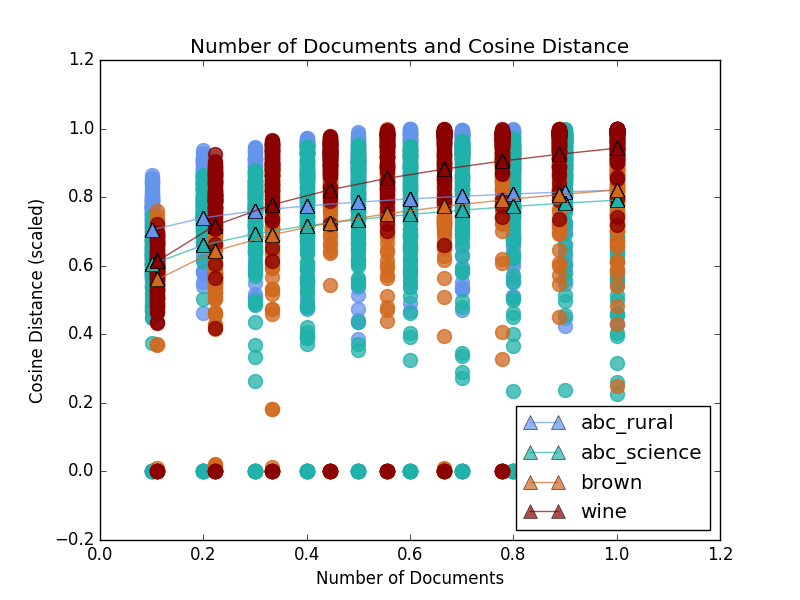
\includegraphics[width=3.0in]{num_docs_cos_fitted.png}
	  }
      \caption{Effect of manipulating number of documents in corpus on cosine distance between topic pairs}
      \label{fig:nd_cos}
\end{figure}

\subsubsection{Jensen-Shannon and Kullback-Leibler Divergence}
Due to their similarity (Kullback-Leibler being the symmetric version of Jensen-Shannon divergence), we show only the results of Kullback-Leibler divergence (KLD). Results show a positive correlation in logarithmic form $y=a*\log(x)+b$ of the divergence between pairs as the number of documents increases.

Increasing document length does not affect the parameters of the scaled relationship. However, increasing stopword presence causes $b$ to decrease for all corpora, as shown in Figure \ref{fig:nd_kld_sw}. This is due to the fact that increasing stopword presence increases the variance in topic scores which draws the best-fit line away from the original mean.

      \begin{figure}[thpb]
      \centering
      \framebox{
      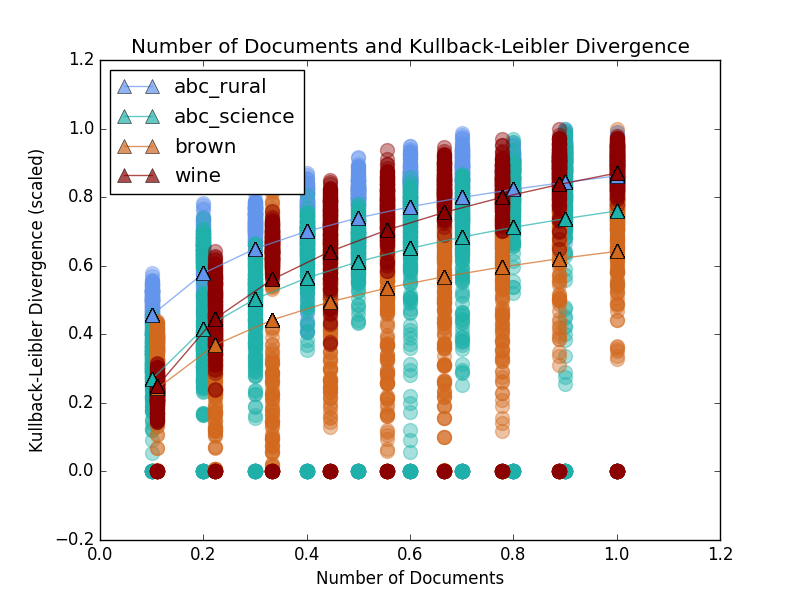
\includegraphics[width=3.0in]{num_docs_kld_fitted.png}
	  }
      \caption{Effect on Kullback-Leibler divergence between topic pairs of manipulating the number of documents in the corpus (the line at the bottom represents topics compared against themselves)}
      \label{fig:nd_kld}
   \end{figure}
   
         \begin{figure}[thpb]
      \centering
      \framebox{
      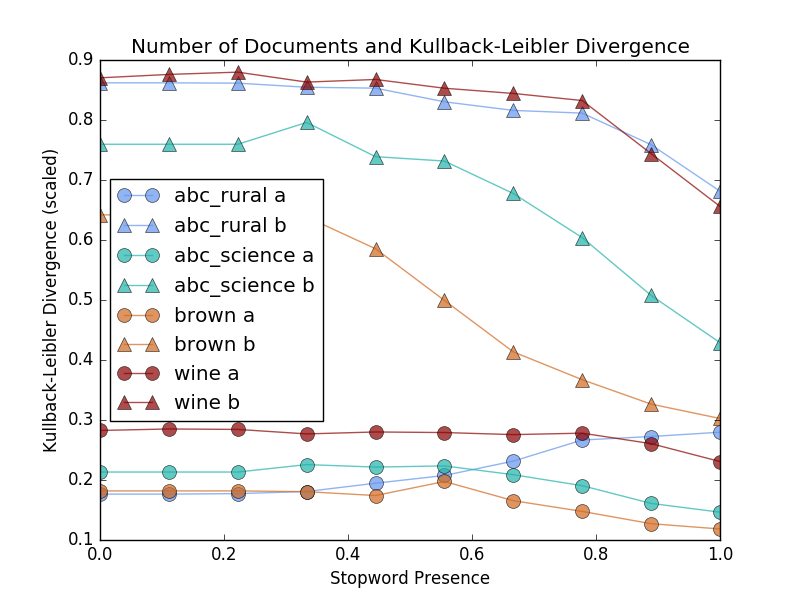
\includegraphics[width=3.0in]{nd_kld_sw.png}
	  }
      \caption{Effect on the relationship between number of documents and resulting Kullback-Leibler divergence between topic pairs of increasing the presence of stopwords in those documents}
      \label{fig:nd_kld_sw}
   \end{figure}

\subsection{Document Length}

\subsubsection{Distance from Uniform Distribution}
Topic distance from the uniform distribution is positively correlated with document length. More-so for the Wine corpus than others. These results are shown in Figure \ref{fig:dl_dist_uni}.

As we increase stopword presence, only Wine shows a brief increase in the correlation coefficient before rapidly dropping to hardly any correlation, with the rest of the corpora. This behaviour can be seen in Figure \ref{fig:dl_dist_uni_sw}.

\begin{figure}[thpb]
      \centering
      \framebox{
      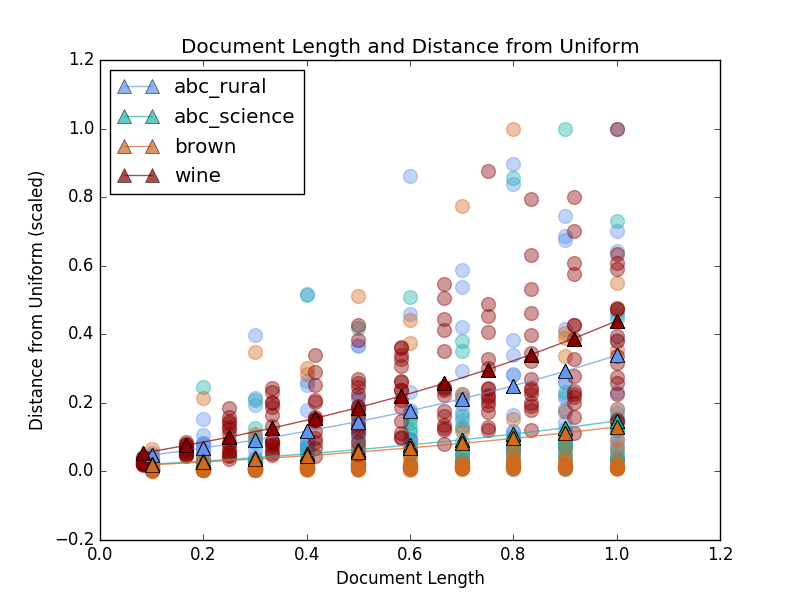
\includegraphics[width=3.0in]{doc_len_dist_uni_fitted.png}
	  }
      \caption{Effect on topic distance from the uniform distribution of increasing document length for each corpus}
      \label{fig:dl_dist_uni}
   \end{figure}
   
  \begin{figure}[thpb]
      \centering
      \framebox{
      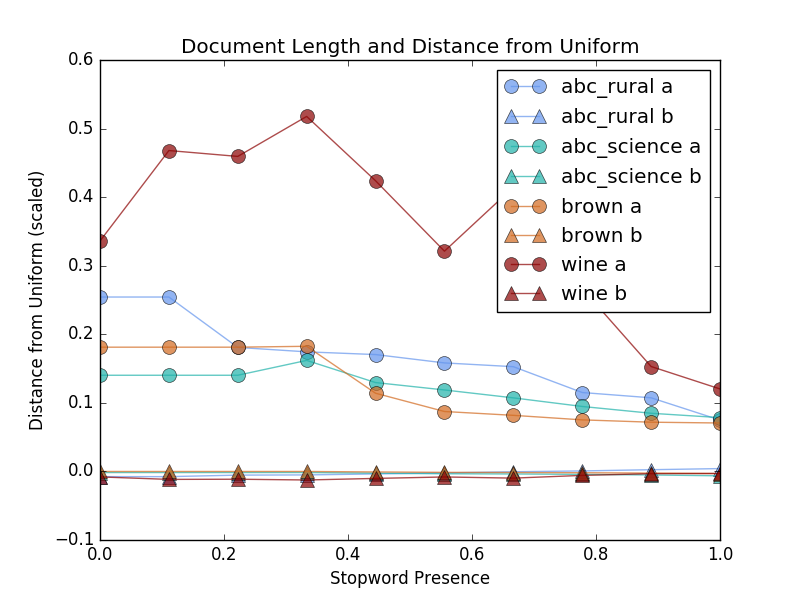
\includegraphics[width=3.0in]{dl_dist_uni_sw.png}
	  }
      \caption{Effect of increasing stopword presence on topic distance from the uniform distribution while increasing document length for each corpus}
      \label{fig:dl_dist_uni_sw}
   \end{figure}
   
\subsubsection{Effective Size}
We observe essentially the relationship between effective size and document length as we do for effective size and number of documents. Results are shown in Figure \ref{fig:dl_eff_size}.
  \begin{figure}[thpb]
      \centering
      \framebox{
      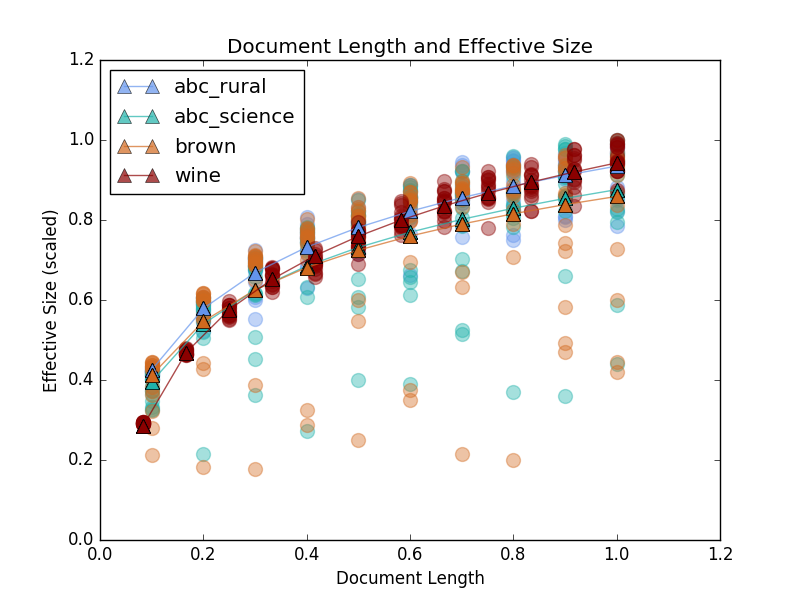
\includegraphics[width=3.0in]{doc_len_eff_size_fitted.png}
	  }
      \caption{Effect of increasing stopword presence on topic distance from the uniform distribution while increasing document length for each corpus}
      \label{fig:dl_eff_size}
   \end{figure}

\subsubsection{Exclusivity}
It is difficult to say, with all of the variation, what specific type of relationship exists between document length and exclusivity. However, it is a positive correlation for all four corpora. Wine is the most affected by changes to document length which makes sense given that this corpus has a mean document length of 25 words to begin with.

\begin{figure}[thpb]
      \centering
      \framebox{
      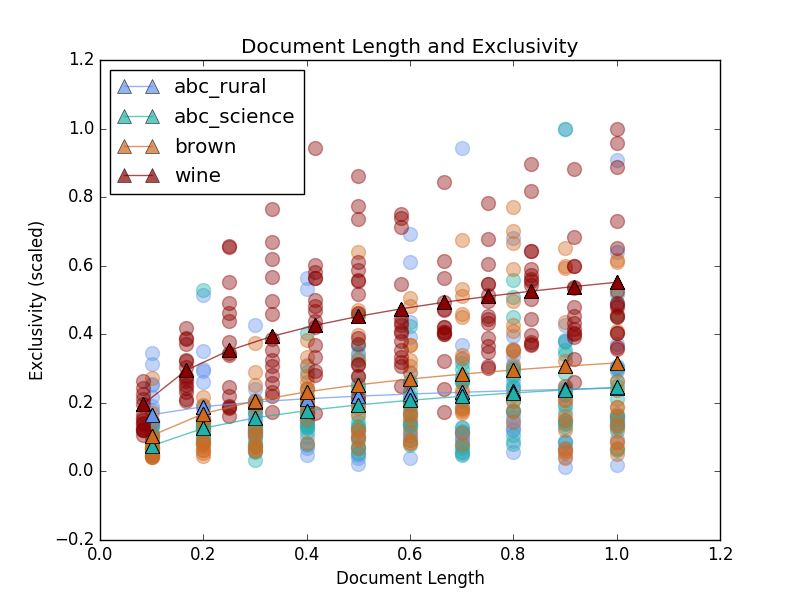
\includegraphics[width=3.0in]{doc_len_exclusivity_fitted.png}
	  }
      \caption{Effect on exclusivity of increasing document length for each corpus}
      \label{fig:dl_exclusivity}
   \end{figure}

\subsubsection{Rank1}
There is no correlation between document length and topic rankings. This result makes sense given the fact that topic rank scores rely significantly on the number of documents in the corpus.

\subsubsection{Cosine Distance}
There is also no correlation between document length and cosine distance of topic pairs.

\subsubsection{Jensen-Shannon and Kullback-Leibler Divergence}
There is a slight positive correlation between topic divergence measured by Kullback-Leibler and Jensen-Shannon divergence. However, there is also significant variety in divergence scores of the various topic pairs.

\begin{figure}[thpb]
      \centering
      \framebox{
      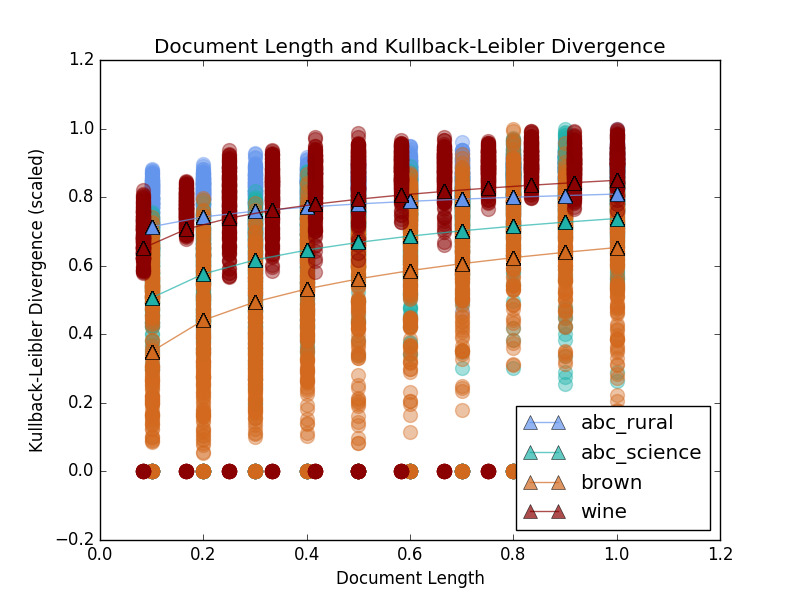
\includegraphics[width=3.0in]{doc_len_kld_fitted.png}
	  }
      \caption{Effect on Rank1 of increasing document length for each corpus}
      \label{fig:dl_kld}
   \end{figure}

\subsection{Stopword Presence}

\subsubsection{Uniform Distribution}
For most topics, distance from uniform distribution decreases as stopword presence is increased. However, for meaningless topics, it increases significantly after 50\% stopword presence. 

\subsubsection{Effective Size}
For the majority of topics, effective size increases relatively slightly as stopword presence is increased. For the corpus-specific stopwords, and other stopwords not captured by our fixed pre-processing, effective size is substantially reduced as the presence of stopwords increases. This behaviour can be seen in Figure \ref{fig:sw_eff_size_4_6} where the corpora have been plotted separately.
\begin{figure}[thpb]
      \centering
      \framebox{
      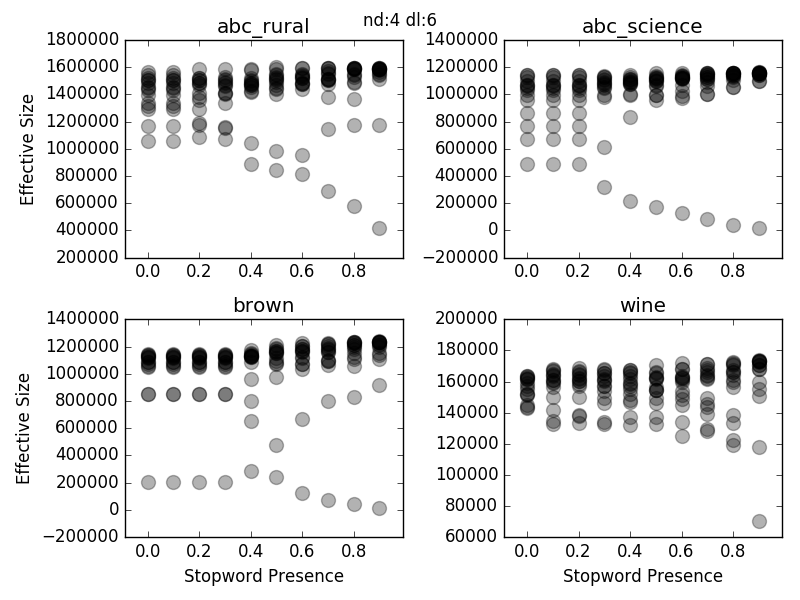
\includegraphics[width=3.0in]{sw_eff_size_4_6.png}
	  }
      \caption{Effect on Rank1 of increasing document length for each corpus}
      \label{fig:sw_eff_size_4_6}
   \end{figure}

\subsubsection{Exclusivity}
Both Wine and ABC Science show a negative correlation (r=-0.3) between stopword presence and topic exclusivity. However, this is largely due to the extremeness of their outliers. The concentration of topic exclusivity scores show no correlation with an increase in stopword presence.

\subsubsection{Rank1}
There is no correlation between stopword presence in documents of any corpus and the resulting topic rankings.

\subsubsection{Cosine Distance}
At smaller values, topic distances diverge to the two possible extremes: very similar or very distinct. Around the natural presence we observed in the original four corpora, the variety in topic similarities begins to increase.

We separate the four corpora for this plot because they exhibit different behaviour after the natural presence threshold, see Figure \ref{fig:sw_cos_8_8}. Brown topics diverges to the two possible extremes. For ABC Rural and Wine, variance in cosine distances begins to increase drastically around 50\% stopword presence. At 90\% stopword presence, unlike Brown, they have converged from the two possible extremes to cover nearly the entire range of possible cosine distance scores. ABC Science remains mostly unaffected. 

\begin{figure}[thpb]
      \centering
      \framebox{
      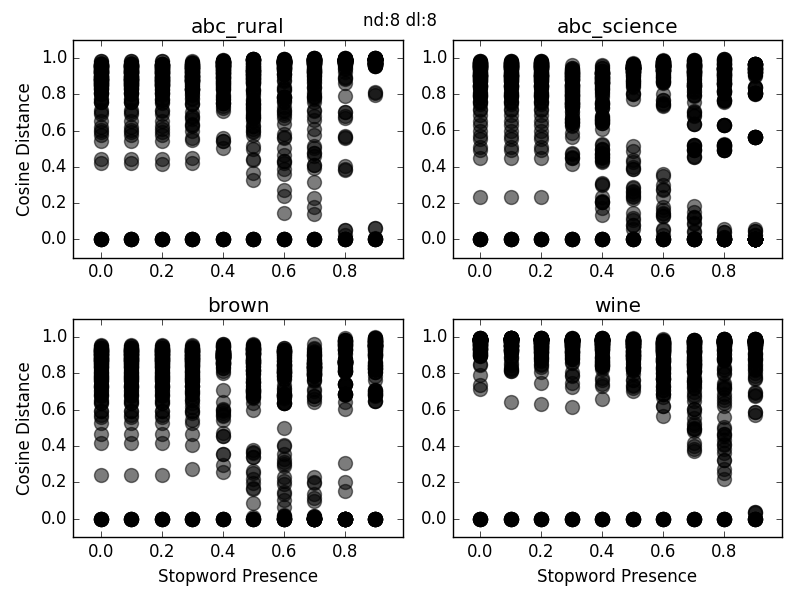
\includegraphics[width=3.0in]{sw_cos_8_8.png}
	  }
      \caption{Effect on Rank1 of increasing document length for each corpus}
      \label{fig:sw_cos_8_8}
   \end{figure}

\subsubsection{Jensen-Shannon and Kullback-Leibler Divergence}
Much like cosine similarity, Jensen-Shannon and Kullback-Leibler divergence showed no impact by stopword removal or injection up to the naturally occurring threshold. Past here, each corpus behaved slightly differently. Their individual characteristics with regards to Jensen-Shannon divergence can be seen in Figure \ref{fig:sw_jsd_4_8}.

\begin{figure}[thpb]
      \centering
      \framebox{
      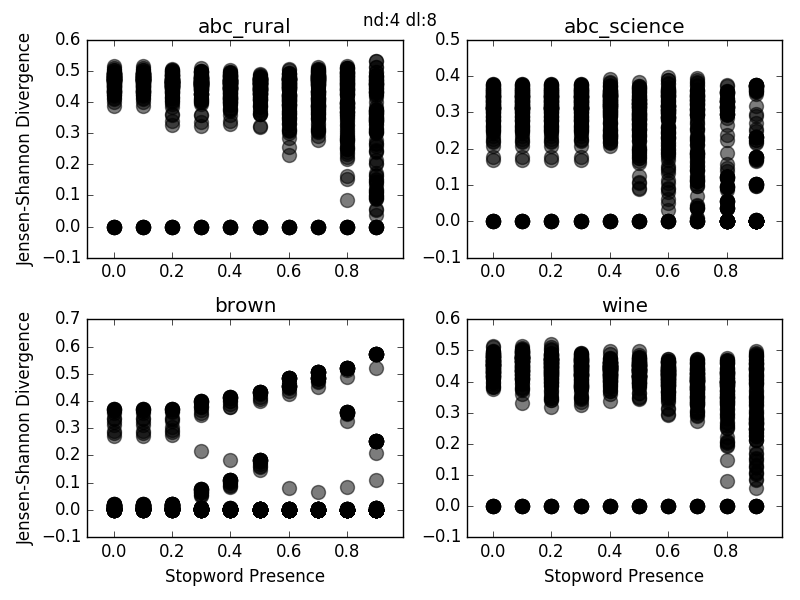
\includegraphics[width=3.0in]{sw_jsd_4_8.png}
	  }
      \caption{Effect on Jensen-Shannon divergence of increasing the stopword presence in each corpus}
      \label{fig:sw_jsd_4_8}
   \end{figure}

\section{DISCUSSION}

\subsection{Corpus Size}
In support of previous findings, we have shown that corpus size plays a large role in topic quality. Our smallest corpus, Wine, was the most affected by changes to document length, document size, and stopword presence. The largest corpus, Brown, was the least affected.

Tang et al. discovered a threshold on the benefits of increasing both document length and number of documents. Although we did not identify the same or different thresholds, we suspect this may be due to the fact that we were not experimenting on as wide a variety of samples. Without wanting to venture too far into the realm of generating synthetic corpora, we were quite limited in finding corpora to experiment on.

The fact that increasing document length does not affect Rank1 scores in any corpus is promising. It means that we did not identify any changes to the most popular topic within any document in the corpus simply by adding or removing words at random from the documents. This finding suggests that documents in existing corpora are robust to some fairly drastic word injection and removal.


\subsection{Stopwords}
Interestingly, we found that stopword presence does not vary much between corpora. Topic similarity as measured by cosine distance remains largely unaffected until stopword injection reaches surpasses this originally observed presence (30-40\%) at which point topics begin to become more similar to one another. Prior to this, the majority of topics have cosine distance greater than 0.5. The few topics less than this are corpus-specific stopwords.

Our most crucial finding is the importance of removing stopwords from a corpus. Unlike some other algorithms, Latent Dirichlet Allocation cannot account for stopwords. Most tutorials will instruct you to choose a list from some obscure online source or use the NLTK list, like in this paper. However, there is no complete list of stopwords and what is considered a ``stopword'' varies from corpus to corpus. Our recommendation is that you filter for stopwords by choosing a large enough K to capture the stopwords, including corpus-specific stopwords, in one or two very poor topics. Since these topics will clearly stand out from the rest when scored with the metrics from this paper, you can easily extract any number of the top words from those poor-scoring topics to use as your list of stopwords.

\subsection{Topic Metrics}
We found that in most cases, our defined topic metrics were enough to distinguish weak topics from strong topics. Future work may need to explore this in more depth. However, the fact that we were able to quickly and easily identify topics containing corpus-specific stopwords means we are headed in the right direction. It would mean a substantial reduction in work load if we could prove that our preliminary findings here hold true for all corpora.

\subsection{Contributions}
Analysis of the results this work results in several contributions. First of all, we confirm the results of related work which has shown the effects of modifying the number of documents and the average document size. In addition, we extend related work by showing the effects of modifying the presence of particular words in the corpus. To our knowledge, this sort of direct approach to modifying a corpus and testing the resulting effectiveness of topic models has not yet been widely studied. Overall, we show that indirectly modifying the underlying vocabulary and word co-occurrences in a corpus reflects natural behaviors and does affect the possibility to effectively model topics within that corpus.

\addtolength{\textheight}{-12cm}   % This command serves to balance the column lengths
                                  % on the last page of the document manually. It shortens
                                  % the textheight of the last page by a suitable amount.
                                  % This command does not take effect until the next page
                                  % so it should come on the page before the last. Make
                                  % sure that you do not shorten the textheight too much.

%%%%%%%%%%%%%%%%%%%%%%%%%%%%%%%%%%%%%%%%%%%%%%%%%%%%%%%%%%%%%%%%%%%%%%%%%%%%%%%%



%%%%%%%%%%%%%%%%%%%%%%%%%%%%%%%%%%%%%%%%%%%%%%%%%%%%%%%%%%%%%%%%%%%%%%%%%%%%%%%%



%%%%%%%%%%%%%%%%%%%%%%%%%%%%%%%%%%%%%%%%%%%%%%%%%%%%%%%%%%%%%%%%%%%%%%%%%%%%%%%%

\section*{ACKNOWLEDGMENTS}

The author thanks Professor David Jensen for his guidance throughout the process of constructing and executing these experiments. She also appreciates his patience with and understanding of her extremely, extreeeeeeeeeemely late submissions.

\bibliographystyle{IEEEtran}
\bibliography{bibi}

% \begin{thebibliography}{99}

% \bibitem{c1} Blei, D. M., Ng, A. Y., and Jordan, M. I. (2003). Latent dirichlet allocation. Journal of machine Learning research, 3 (Jan), 993-1022.
% \bibitem{c2} Mimno, D., and McCallum, A. (2007, June). Organizing the OCA: learning faceted subjects from a library of digital books. In Proceedings of the 7th ACM/IEEE-CS joint conference on Digital libraries (pp. 376-385). ACM.
% \bibitem{c3} Tang, J., Meng, Z., Nguyen, X., Mei, Q., and Zhang, M. (2014, January). Understanding the limiting factors of topic modeling via posterior contraction analysis. In International Conference on Machine Learning (pp. 190-198).
% \bibitem{c4} Zhao, W. X., Jiang, J., Weng, J., He, J., Lim, E. P., Yan, H., and Li, X. (2011, April). Comparing twitter and traditional media using topic models. In European Conference on Information Retrieval (pp. 338-349). Springer, Berlin, Heidelberg.
% \bibitem{c5} 

% \end{thebibliography}

\end{document}
